
\chapter{\LaTeX{} 与 Word 比较}{Compare \LaTeX with Word}
\LaTeX{}\index{\LaTeX} 与 Word 是两种不同类型的文本编辑处理系统, 各有所长, 如果要对文字编辑性能
和使用便捷程度等作综合评比, Word 明显优于 \LaTeX\index{\LaTeX}, 仅``所见即所得"一项, Word 就会
赢得绝大多数用户, 但要仅限定在学术报告和科技论文方面, 评比结果就不同了.

\section{从头开始}{From the Beginning}

Word 特点就是``所见即所得", 其基本功能初学者很容易掌握, 很多 Word 用户都是无师自
通. 但随着篇幅和复杂程度的增加, 花费在文稿格式上的精力和时间要明显加大, 如图
\ref{fig:CompareWithWord} 蓝
色示意曲线所示. 因为创建自定义编号、交叉引用、索引和参考文献等就不是``所见即所得"
了, 得耐着性子反复查阅 Word 的在线帮助或借助相关软件帮忙.

对于 \LaTeX{}\index{\LaTeX} 初学者, 即就是编排很简单的文章, 也要花较多的精力和时间去学习那些
枯燥的命令和语法, 特别是排写数学公式, 经常出错, 多次编译不能通过, 使很多初学者望
而却步. 可是一旦掌握, 不论文稿长短和复杂与否都会熟练迅速地完成, 先前学习 \LaTeX{}\index{\LaTeX}
的精力投入将由此得到回报, 如图 \ref{fig:CompareWithWord} 红色示意曲线所示.

\begin{figure}
  \centering
  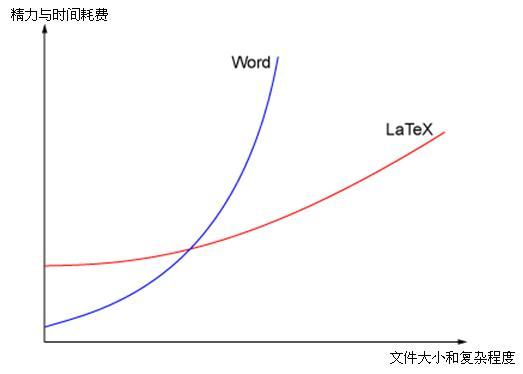
\includegraphics[width=9cm]{CompareWithWord.jpg}\\
  \caption{与 Word 比较}{Compare with Word}\label{fig:CompareWithWord}
\end{figure}

\section{内容与样式}{Contents and Format}
当用 Word 写作时, 要花很多精力对页版式、章节样式、字体属性、对齐和行距等文本参数进
行反复选择对比, 尤其是长篇文章, 经常出现因疏忽而前后文体格式不一致的现象; 当在稿件
中插入或删除一章或章节次序调整时, 各章节标题、图表和公式等的编号都要用手工作相应修
改, 稍有不慎就会出现重号或跳号. 你既是作者又是编辑还兼排字工.

使用 \LaTeX{}\index{\LaTeX} 编版, 如无特殊要求, 只要将文稿的类型 (article, report 或 book 等) 告
诉 \LaTeX\index{\LaTeX}, 就可专心致志地写文章了, 至于文稿样式的各种细节都由 \LaTeX{}\index{\LaTeX} 统一规划设
置, 而且非常周到细致; 当修改稿件时, 其中的章节、图表和公式等的位置都可任意调整, 无
须考虑编号, 因为在源文件里就没有编号, 文件中的所有编号都是在最后编译时 \LaTeX{}\index{\LaTeX} 自
动统一添加的, 所以绝对不会出错.

换句话说, Word 把文稿的内容与样式混为一体, 而 \LaTeX{}\index{\LaTeX} 将它们分离, 作者只需专注于
文稿的内容, 而文稿的样式几乎不用过问, \LaTeX{}\index{\LaTeX} 是你的聪明而忠诚的文字秘书, 如有特
殊要求, 也可使用命令修改, \LaTeX{}\index{\LaTeX} 会自动将相关设置更新, 无一遗漏.

接受 \LaTeX{}\index{\LaTeX} 稿件的出版社大都有自己的文稿样式模板, 主要就是一个类型文件包, 简称类
包. 如果稿件未被甲出版社采用, 在转投乙出版社前, 只需将稿件第一句中类包名称由甲出版
社的改为乙出版社的, 整篇稿件的样式就随之自动转换过来了. 就一句话的事儿, 简单的不能
再简单了, 然而因为``体制"的原故, Word 却根本无法做到这一点.

\section{数学公式}{Mathematical Formulas}
Word 有个公式编辑器, 可以编辑普通数学公式, 但使用很不方便, 外观效果较差, 也不能自
动编号, 尤其是很难作为文本的一部分, 融入某一行中, 大都专起一行. 如果碰到复杂的数学
公式, 编辑起来就很困难. 有些用户只好另外安装可嵌入 Word 环境的工具软件 MathType 来
弥补这一不足.

\LaTeX{}\index{\LaTeX} 的特长之一就是数学公式编辑, 方法简单直观, ``所想即所得", 公式的外观精致细
腻, 而且公式越复杂这一优点就越明显. 普通单行公式可以像纯文字文本一样插入字里行间.
下面举三例加以比较 (如图 \ref{fig:CompareTheDisplayOfWordAndLaTeX}), 其中 Word 分两
种情况, 一是 DOC 格式的屏幕显示效果, 二是将 DOC 格式文件通过 Acrobat 转换为 PDF 格
式的效果.

\begin{figure}
  \centering
  \begin{tabu}to.7\linewidth{X[1rm]X[1.5lm]}
    Word: & 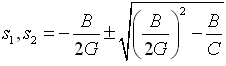
\includegraphics[width=5cm]{WordFormula.png}\\
    Word 转化为 PDF: & 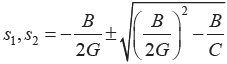
\includegraphics[width=5cm]{WordFormulaInPDF.png}\\
    \LaTeX{}: & $s_1$, $\displaystyle s_2=-\frac{B}{2G}\pm\sqrt{\left(\frac{B}{2G}\right)^2-\frac{B}{C}}$\\
  \end{tabu}
  \caption{Word 与 \LaTeX{}\index{\LaTeX} 公式显示效果对比}{Compare the display of Word and \LaTeX}
  \label{fig:CompareTheDisplayOfWordAndLaTeX}
\end{figure}

Word 在某些时候公式会出现对接不齐, 行距变宽等现象, 而 \LaTeX{}\index{\LaTeX} 编辑的公式在整个文档
中一直对接工整, 行距不变, 如图 \ref{fig:CompareTheAlignOfWordAndLaTeX}.

\begin{figure}
 \centering
 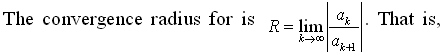
\includegraphics[width=9cm]{WordFormulaNotAlign.png}\\
 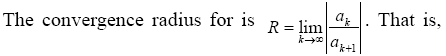
\includegraphics[width=9cm]{WordFormulaNotAlignInPDF.png}\\
 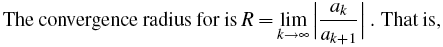
\includegraphics[width=9cm]{LatexFormulaAlign.png}\\
 \caption{Word 与 \LaTeX{}\index{\LaTeX} 公式的对齐比较}{Compare the align of Word and \LaTeX{}}
 \label{fig:CompareTheAlignOfWordAndLaTeX}
\end{figure}

尽管在默认状态下, 就能将数学公式编排的非常精致美观, \LaTeX{}\index{\LaTeX} 仍然还提供了很多调节
命令, 可以对公式的外观作更加细微的调整, 使其尽善尽美.

\section{插图}{Figures}

Word 有个绘图工具, 简易直观, 但功能有限效果不佳. 论文中的复杂图形大都用功能强大的
Visio、Photoshop 等绘图软件绘制, 然后插入 Word.

\LaTeX{}\index{\LaTeX} 自身也具有简单的绘图功能, 如调用各种绘图宏包, 可画出非常复杂的图形, 缺点
是不直观, 命令格式繁琐, 不易熟练掌握, 名曰画图, 实为编程. 可同样先使用 Visio 绘图,
然后粘贴到 Adobe Illustrator, 对图形的细节作进一步处理后, 存储为 PDF 或 EPS 格式,
最后用插图命令调入 \LaTeX{}\index{\LaTeX} 源文件即可, 其效果更为精致.

\section{创建参考文献}{Management References}

Word 目前还不具备管理参考文献的功能, 用户一般都是采用 Reference Manager 或是
NoteExpress 等外部工具软件来解决这一问题.

创建参考文献可是 \LaTeX{}\index{\LaTeX} 的强项. \LaTeX{}\index{\LaTeX} 自带一个辅助程序 BibTeX, 它可以根据作者
的检索要求, 搜索一个或多个文献数据库, 然后自动为文稿创建所需的参考文献条目列表. 如
果编写其它文件用到相同的参考文献时可直接引用这个数据库. 参考文献的样式和排序方式都
可以自行设定.

很多著名的科技刊物出版社、学术组织和 TUG 网站等都提供相关的 BibTeX 文献数据库文件,
可免费下载.

\section{显示与输出}{Display and Output}

在文本对齐、字体变换、拼写检查、单词间距控制、自动断词和自动换行等纯文字处理功能方
面, Word 经多次升版后已与 \LaTeX{}\index{\LaTeX} 相差无几, 但是排版效果却有所不同. 以 Times 字体
为例, 在 Word 中``Ta"和``PA"两个字母的间距有些松散, 见下图所示. \LaTeX{}\index{\LaTeX} 将各种拼写
组合时的字母间距进一步优化调整, 松紧得当, 使整个文本的排版效果更加工整匀称.

\begin{figure}
  \centering
  \begin{tabu}spread 1mm{X[-1rm]X[lm]}
    Word:\par\LaTeX: & 
\includegraphics[width=4cm]{WordPanda.pdf}\\
  \end{tabu}\vskip-5pt
\end{figure}

在换行时, \LaTeX{}\index{\LaTeX} 不仅可以根据音节自动断词, 也可以按照作者的要求进行设定断词, 一
个单词可以设定多种断词方式, 特别适用于科技论文中反复出现的专业词汇或缩略写, 这既能
保持单词间距均匀, 又不易产生误解.

在科技著作手稿中经常可以看到某些论述附有说明、出处或考证; 或者某些段落划上黑杠以示
删除; 或在边空里写有准备补充的文字. 在 \LaTeX{}\index{\LaTeX} 源文件中使用注释标记可以将上述这些
内容完整地保留下来, 以备后用, 而在编译后的 PDF 文件中还看不到这些内容. 科研论文要
经过反复推敲, 多次修改, 注释功能非常实用. ``所见即所得"的 Word, 当然没有这个功能,
它删除的内容就甭想再找回来了.

一篇论文, Word 新手与牛人的排版美观程度差别很大, ``所见即所得"成了一大缺点, 因为
Word 本身不能帮助作者美化作品, 自己排成什么样就什么样, 即: ``所得仅所见", 就像在白
纸上作画, 全凭个人的悟性与灵感. 而 \LaTeX{}\index{\LaTeX} 初学与专家的排版外观差别很小, 仅是快慢
不同, 都能达到专业出版水平, 这就是 \LaTeX{}\index{\LaTeX} 的一大优点, 只要想法一致就能得到相同的
结果, 即``所想即所得".

目前 PDF 格式已成为全世界各种组织机构用来进行更加安全可靠的电子文件分发和交换的出版
规范, 科技论文大都使用 PDF 格式. \LaTeX{}\index{\LaTeX} 可以直接输出 PDF、PS 或 DVI 格式文件; 而
Word 输出的是 DOC 格式文件, 还须购买 Adobe Acrobat 软件, 将 DOC 转换为PDF; 另外, 图
形中的数学公式或文本中数学式的上下标, 在转换后常出现位置偏移字形变大等问题.

\section{可扩充性}{Expansible}

用户可以像搭积木那样对 \LaTeX{}\index{\LaTeX} 进行功能扩充或添加新的功能. 例如, 加载一个 CJK 宏
包, 就可以处理中文, 调用 eucal 宏包可将数学公式中的字符改为欧拉书写体; 如果对某个
宏包效果不太满意, 完全可以打开来修改, 甚至照葫芦画瓢自己写一个. 这些可附加的宏包
文件绝大多数都可从 CTAN 等网站无偿下载.

因为设计的超前性, \TeX/\LaTeX{}\index{\LaTeX} 程序系统几十年来没有什么改动, 而且由于它的可扩充性,
\LaTeX{}\index{\LaTeX} 将永葆其先进性, 也就是说, 学习和使用 \LaTeX{}\index{\LaTeX} 永远不会过时. 例如, 通过调用
相关扩展宏包, \LaTeX{}\index{\LaTeX} 立刻就具备了排版高质量高专业水准象棋谱、五线谱或化学分子式
的能力. 对于 \LaTeX{}\index{\LaTeX} 这种机动灵活、简便免费的可扩充性能, Word 只能望尘.
